\documentclass[11pt]{article}

\usepackage[T1]{fontenc}
\usepackage[utf8]{inputenc}
\usepackage[margin=1in]{geometry}
\usepackage{booktabs}
\usepackage{graphicx}
\usepackage{amsmath}
\usepackage{amssymb}
\usepackage{url}
\usepackage[hidelinks]{hyperref}

\graphicspath{{../experiments/plots/}}
\emergencystretch=3em

\title{\bfseries Trace-Count Thresholds and Implementation-Runtime Effects in
AES-128 Final-Round Cache-Collision Key Recovery:\\
A Controlled C, Go, and Python Study}

\author{}
\date{}

\begin{document}
\maketitle

\begin{abstract}
\noindent
Table-driven software implementations of AES leak secret-dependent information
through cache timing. The Bonneau--Mironov final-round cache-collision attack
turns this leak into key recovery by grouping traces on ciphertext-byte
differences. Because such recovery is statistical, a central practical question
is \emph{how many traces} are required---and whether that number depends on the
\emph{language} in which the vulnerable target and its measurement loop are
written. We study both questions in a controlled, local AES-128 laboratory with
three independent implementations (C, Go, Python) that share one attack pipeline
and one fixed key. On an Apple M4, the C implementation recovers and
cryptographically verifies the key with a fitted 50\% threshold of
$N_{50}\approx 51{,}346$ traces ($2^{15.6}$); flat per-trace timing statistics
show the threshold is an averaging effect, not a signal cliff. Collecting the
\emph{same} attack's traces in Go's managed runtime raises the threshold about
five-fold ($N_{50}\approx 265{,}000$). A garbage-collector ablation
(\texttt{GOGC=off}, \texttt{GOMAXPROCS=1}) localises the cause: disabling the
collector shifts the threshold by under 8\% and does not close the gap, so the
disadvantage is broad runtime measurement \emph{noise}, not GC pauses. After
normalising the three ports' timer units, Go's mean per-encryption cost is only
$\approx 2.4\times$ C's, confirming that the five-fold threshold gap is driven by
timing \emph{variance} rather than mean overhead. Pure-Python collection and
recovery are $\approx 55\times$ and $\approx 1800\times$ slower than C, making a
full measured characterisation take on the order of weeks and placing verified
recovery beyond any feasible trace budget. The study contributes a
statistically grounded threshold estimate, the first controlled cross-language
measurement of that threshold in this setting, and evidence that implementation
runtime---not only the algorithm---shapes the practical cost of a cache-timing
attack.
\end{abstract}

% ===========================================================================
\section{Introduction}
\label{sec:intro}

The Advanced Encryption Standard (AES) is a widely deployed symmetric block
cipher standardised by NIST~\cite{fips197}. Its mathematical design resists
practical exhaustive search and conventional cryptanalysis at appropriate key
sizes. In practice, however, the security of a cryptographic system depends not
only on the cipher but on how the cipher is implemented, compiled, and executed.
A software implementation can reveal information through observable behaviour
such as execution time, memory-access patterns, power, or electromagnetic
emissions; these implementation-dependent observations are called side channels.

Timing attacks are an important class of side-channel analysis. Kocher showed
that execution-time variation can reveal secret information when the cost or
sequence of operations depends on private values~\cite{kocher96}. Such attacks
are statistical rather than deterministic: many observations are collected,
candidate hypotheses are scored, and the best-explaining hypothesis is
preferred. A single measurement rarely suffices because runtime also reflects
scheduling, interrupts, cache replacement, memory contention, frequency scaling,
and timer overhead.

Processor caches are especially relevant to software cryptography. Historical
high-performance AES implementations used lookup tables indexed by intermediate
state bytes; because those bytes depend on the input and the round key, the
table-access pattern---and hence cache behaviour---can depend on the secret key.
Bernstein demonstrated that aggregate timing leaks information from table-based
AES~\cite{bernstein05}; Bonneau and Mironov presented a cache-collision timing
attack that infers relations among final-round key bytes from relations among
ciphertext bytes~\cite{bonneau06}; Osvik, Shamir, and Tromer described
access-driven cache attacks and countermeasures~\cite{osvik06}.

This paper studies a controlled AES-128 cache-timing laboratory inspired by that
line of work. The target is intentionally vulnerable and table based; it is not
a modern production library. Its purpose is to make the leakage mechanism
observable, to support repeatable statistical experiments, and to allow the
entire recovery process---from trace collection to cryptographic key
verification---to be inspected. The laboratory contains independent
implementations in C, Go, and Python. C offers direct memory control and low
overhead; Go is compiled but runs within a managed runtime with automatic memory
management and bounds checks; Python is a concise, readable interpreter. These
differences let us ask not only \emph{how many traces} the attack needs, but
whether that number changes with the implementation collecting them.

The empirical focus is the \textbf{measured trace-count threshold}: because
recovery has a probability rather than a fixed boundary, estimating the
transition from likely failure to likely success is central to evaluating the
attack. We then hold the algorithm fixed and vary only the implementation to
isolate the effect of the runtime on that threshold.

\paragraph{Contributions.}
\begin{enumerate}
  \item A statistically grounded estimate of the measured trace-count threshold
        for the final-round cache-collision attack on an Apple M4
        ($N_{50}\approx 51{,}346$; high reliability near $75$k), with evidence
        (flat \texttt{min\_time} and score across count) that the threshold is a
        statistical averaging effect rather than a signal cliff
        (Sec.~\ref{sec:res-threshold}, \ref{sec:an-statistical}).
  \item A controlled \emph{native-collection} cross-language comparison showing
        that collecting the same attack's traces in Go's managed runtime raises
        the threshold about fivefold, to $N_{50}\approx 265{,}000$
        (Sec.~\ref{sec:res-crosslang}).
  \item A garbage-collector ablation that localises the cause: quieting the Go
        runtime moves the threshold by $<8\%$ and does not close the gap, so the
        gap is broad measurement noise, not the collector
        (Sec.~\ref{sec:res-gc}, \ref{sec:an-crosslang}).
  \item A timer-unit-normalised cost comparison (C, Go, Python) separating
        \emph{mean} per-encryption overhead ($\approx 2.4\times$ for Go,
        $\approx 420\times$ for Python) from the timing \emph{variance} that
        actually drives the threshold (Sec.~\ref{sec:res-cost},
        \ref{sec:an-crosslang}).
  \item A feasibility bound showing pure-Python measured recovery is impractical
        on this platform---a full characterisation would take on the order of
        weeks and its noisier timer implies a threshold beyond any feasible
        trace budget (Sec.~\ref{sec:res-python}, \ref{sec:an-python}).
  \item An open, auditable methodology with explicit dataset-governance and
        exclusion criteria (Sec.~\ref{sec:method-governance}, Appendix~\ref{app:prov}).
\end{enumerate}

\paragraph{Research questions.}
\begin{description}
  \item[RQ1] How does trace count affect the probability that the measured
        attack reconstructs and verifies the original AES-128 key?
  \item[RQ2] Holding the algorithm, key, and parameters fixed, does the
        implementation language collecting the traces change recovery
        reliability and the trace threshold?
  \item[RQ3] If Go requires more traces than C, is the difference caused by the
        garbage collector, or by broader runtime timing noise?
  \item[RQ4] What is the cross-language cost of collection and recovery, and is
        pure-Python measured recovery feasible at all?
\end{description}
A complementary question---whether the three implementations recover an
\emph{identical} key from one \emph{shared} trace file (algorithmic
consistency), and their stage-level processing times on that shared
input---is deliberately left to future work (Sec.~\ref{sec:conclusion}); the
experiments here concern native, per-implementation collection.

% ===========================================================================
\section{Background}
\label{sec:background}

\subsection{AES-128 and the final round}
AES-128 operates on a 128-bit block (16 bytes) with a 128-bit key. After an
initial key addition it performs ten rounds; the first nine apply SubBytes,
ShiftRows, MixColumns, and AddRoundKey, while the tenth omits
MixColumns~\cite{fips197}. This simpler final round supports a direct relation
between ciphertext bytes and tenth-round key bytes. Let $C_i, C_j$ be two
ciphertext bytes and $K^{(10)}_i, K^{(10)}_j$ the corresponding tenth-round key
bytes. Under the exact-collision model implemented here, two relevant final-round
lookup inputs collide when $C_i \oplus K^{(10)}_i = C_j \oplus K^{(10)}_j$, i.e.
\begin{equation}
C_i \oplus C_j = K^{(10)}_i \oplus K^{(10)}_j .
\label{eq:collision}
\end{equation}
The left side is computable from observed ciphertext; the right side is the XOR
relation between two unknown key bytes.

\subsection{Pairwise timing model and relative-key recovery}
For a position pair $(i,j)$, define $\Delta_{i,j}=C_i\oplus C_j$, which takes 256
values. Traces are grouped by $\Delta_{i,j}$ and each group's mean timing is
computed; the group satisfying Eq.~\eqref{eq:collision} receives more relevant
collisions and a lower average timing. With 16 ciphertext bytes there are
$\binom{16}{2}=120$ pairs, giving 120 timing tables of 256 entries. A candidate
\emph{relative} key $R=(R_0,\dots,R_{15})$ is scored globally,
\begin{equation}
S(R)=\sum_{0\le i<j<16} T_{i,j}[R_i\oplus R_j],
\label{eq:score}
\end{equation}
where $T_{i,j}[d]$ is the mean timing for difference $d$; lower is better.
Multi-start coordinate descent minimises $S$. The relative key fixes all pairwise
XORs but leaves one common offset $x$: $K^{(10)}_i = R_i \oplus x$. Enumerating
$x\in\{0,\dots,255\}$, reversing the AES-128 key schedule, and testing each
candidate against a stored plaintext--ciphertext pair yields an objective,
verified recovery. A low score is never counted as success unless the candidate
passes this cryptographic check.

\subsection{Synthetic and measured timing}
The laboratory provides two timing modes. \emph{Synthetic} mode generates a
timing value from a modelled collision signal plus noise, validating the attack
logic independently of hardware. \emph{Measured} mode records elapsed time around
the vulnerable target: before each timed operation it reads a configurable memory
buffer to disturb the cache, then repeats the encryption several times and
accumulates the duration into one trace. Repetition raises the target's
contribution relative to fixed timer overhead, though environmental noise
remains.

% ===========================================================================
\section{Related Work}
\label{sec:related}

Kocher introduced timing attacks against public-key
implementations~\cite{kocher96}. For AES specifically, Bernstein showed that
aggregate end-to-end timing of a network server leaks key
information~\cite{bernstein05}; his attack is powerful but data-hungry, and
Neve, Seifert, and Wang, refining Bernstein's analysis, report on the order of
$2^{18}$--$2^{21}$ samples across processors~\cite{neve06}. Osvik, Shamir, and
Tromer developed \emph{access-driven} attacks in which a spy process observes
cache state directly, recovering a key from as few as $\sim$800 encryptions in a
synchronous setting, and surveyed countermeasures~\cite{osvik06}; that model
assumes co-resident cache observation rather than timing alone.

The attack implemented here follows Bonneau and Mironov's
\emph{cache-collision} model~\cite{bonneau06}, which exploits relations among
ciphertext bytes (Eq.~\eqref{eq:collision}) using only timing. Their expanded
final-round attack reports a \emph{median} of $2^{13}$--$2^{14.3}$ samples under
cache eviction on 2006-era Pentium III/UltraSPARC hardware.

All of this prior work characterises a \emph{single} implementation on
period-specific hardware. Our contribution is orthogonal to the attack itself:
we quantify the measured trace threshold on modern hardware with statistical
confidence intervals, and---holding the algorithm fixed---measure how the
\emph{implementation runtime} that performs the collection changes that
threshold. To our knowledge this cross-language, same-pipeline comparison, and
the accompanying garbage-collector ablation, have not previously been reported.

% ===========================================================================
\section{Methodology}
\label{sec:method}

\subsection{Research design}
The study combines four linked components. \textbf{(A) Threshold estimation}: the
measured C collector generates datasets at multiple trace counts while key,
repetition, eviction size, filtering, recovery algorithm, and verification stay
fixed; recovery success is modelled as a probability over ten trials per count.
\textbf{(B) Native cross-language recovery}: C and Go each perform their own
measured collection and recovery under identical parameters, and we compare
recovery reliability versus count. \textbf{(C) Garbage-collector ablation}: the
Go collection is repeated with the runtime quieted. \textbf{(D) Cross-language
cost and Python feasibility}: per-stage timing is measured for all three ports
and extrapolated. The pipeline is
Validate~$\rightarrow$~Collect/Load~$\rightarrow$~Filter~$\rightarrow$~Group~$\rightarrow$~Estimate~$\rightarrow$~Enumerate~$\rightarrow$~Reverse~$\rightarrow$~Verify.

\subsection{Environment and reproducibility}
All runs execute on an Apple M4 (10 logical cores, 16\,GiB, Darwin arm64) at
source commit \texttt{405b3de} with the experiment harness modified in place
(the attack sources unchanged). Each run records a UTC timestamp, commit,
processor, memory, parameter values, randomised run order, and seed. One fixed
128-bit AES key is generated once and reused throughout so that trace count,
dials, and implementation are the only variables. Runs are interleaved across
(count,\,trial) pairs using a seeded Fisher--Yates shuffle: grouped execution
would let a transient load event bias an entire condition, whereas interleaving
spreads such noise across conditions while remaining reproducible.

\subsection{System validation}
Before interpreting measured timing we validate, in stages, that (1) AES-128
encryption matches a NIST test vector; (2) the table-based target is functionally
equivalent to a reference AES; (3) the reverse key schedule is correct; (4) the
full attack recovers keys from synthetic timing; and (5) candidates are checked
with the stored verifier pair. Staged validation is necessary because a failed
measured attack can arise from insufficient signal, an implementation error, an
incorrect final-round relation, a scoring error, local-search failure, or faulty
key-schedule reversal; separating these reduces ambiguity.

\subsection{Timing-trace collection and instrumentation}
\label{sec:method-collect}
For each trace the collector generates a random 16-byte plaintext, reads a
2048\,KiB memory region to disturb the cache, starts a timer, repeats the
vulnerable encryption 50 times, stops the timer, and stores the plaintext,
ciphertext, and aggregate duration. The recorded value is an aggregate elapsed
time; individual cache events are not recorded.

The three ports use different clocks, which matters for any cross-language
timing comparison (Sec.~\ref{sec:res-cost}). C reads
\texttt{mach\_absolute\_time()}, whose Apple-Silicon timebase is 24\,MHz, so one
tick is $1/24\,\mathrm{MHz}\approx 41.67$\,ns. Go uses
\texttt{time.Since().Nanoseconds()} and Python uses
\texttt{time.perf\_counter\_ns()}, both already in nanoseconds. We convert C ticks
to nanoseconds before any cross-language magnitude comparison; recovery-rate
comparisons are unaffected because each implementation's filter and score are
computed in its own consistent units.

\subsection{Filtering, tables, optimisation, verification}
Before building tables, timings satisfying $t>2\,t_{\min}$ (with $t_{\min}$ the
per-dataset minimum) are excluded to bound the effect of scheduling outliers on
group means; the rule is a heuristic and the used/ignored counts are recorded for
audit. Pairwise tables are built per Eq.~\eqref{eq:score}; the global score is
minimised by multi-start coordinate descent; the common offset is enumerated over
256 values; and each candidate is verified cryptographically. Each trial's
outcome is therefore binary: verified recovery or not.

\subsection{Statistical analysis}
\label{sec:method-stats}
At each count the empirical recovery rate is $\hat p=k/n$ with $n=10$. Because ten
trials leave substantial uncertainty near 0\% and 100\%, we report 95\% Wilson
score intervals. A logistic model $\Pr(\text{success}\mid N)=\sigma(a+b\log_2 N)$
is fitted to trial-level outcomes by iteratively reweighted least squares with a
small ridge term for numerical stability, giving a 50\% threshold
$N_{50}=2^{-a/b}$; a model-independent linear interpolation in $\log_2 N$ space
provides a consistency check.

\subsection{Dial sweep and its fixed count}
\label{sec:method-dial}
A complementary experiment holds count fixed and varies the two collection dials
to separate \emph{averaging} from \emph{signal strength}: \texttt{-repeat} $r$
(encryptions accumulated per trace) and \texttt{-evict-kb} $e$ (cache-disturbance
buffer size). The count is fixed at \textbf{100{,}000 traces}, chosen
deliberately in the C attack's marginal region just above $N_{50}$
(Sec.~\ref{sec:res-threshold}), where recovery is most sensitive to signal
quality; a count deep in the reliable ($100\%$) or failure ($0\%$) regime would
mask any dial effect. We sweep $r\in\{10,20,30,50,75,100\}$ and
$e\in\{256,512,1024,2048,4096\}$\,KiB about the $r{=}50,\,e{=}2048$ baseline, ten
interleaved trials each.

\subsection{Native cross-language collection and its confound}
\label{sec:method-crosslang}
Each implementation performs its \emph{own} measured collection with its native
timer and then runs its own recovery; we compare recovery reliability versus
count. Trace count, the fixed key, dials, filtering, recovery algorithm, and
verification are identical; only the implementation (hence its collection
runtime) changes. Because each language collects independently, the trace data
and its random seed differ across implementations---so a difference in recovery
is attributable to the language's runtime behaviour during collection, not to the
common attack logic. This is a native-collection comparison and is kept distinct
from a shared-dataset consistency test.

\subsection{Garbage-collector ablation}
\label{sec:method-gc}
To test whether Go's managed runtime causes its higher threshold, the Go
collection is repeated with \texttt{GOGC=off} (no collector, hence no GC pause
inside a timed region) and \texttt{GOMAXPROCS=1} (one core, suppressing
cross-core migration); both are read from the environment with no source change.
For cost, the ablation uses a reduced grid (counts $\{500,250,100,50\}$k and a
$3\times3$ dial grid) and is compared to the collected run only at matched counts
and by fitted $N_{50}$.

\subsection{Cross-language cost and Python feasibility protocol}
\label{sec:method-python}
On an idle machine we time \texttt{collect-real} and \texttt{attack-final} for
each port at small counts (removing fixed start-up by taking the marginal slope
between two counts), yielding per-sample collection and attack costs and, from
each port's $t_{\min}$, a per-encryption time normalised to nanoseconds. From
these we extrapolate the wall-clock cost of representative Python recovery
workloads to assess feasibility.

\subsection{Dataset governance and exclusion criteria}
\label{sec:method-governance}
Several exploratory runs preceded the retained runs; to avoid selective
reporting, inclusion follows fixed rules and every excluded run's metadata is
preserved (Appendix~\ref{app:prov}). \textbf{Environment gate}: exclude any run
whose mean collection cost exceeds $\approx1.2$\,ms/sample (baseline
$\approx0.94$), a proxy for background load; one 10-trial C sweep is excluded on
this basis ($\approx3.0$\,ms/sample). \textbf{Design gate}: pilots with fewer
trials, missing sidecars, or single-point grids are used only for design context.
\textbf{Implementation identity}: one retained C run was launched with an
\texttt{IMPL=go} tag \emph{before} the harness supported language selection, so
the C binary in fact executed; it is verified as C (no \texttt{impl} field in its
metadata; $t_{\min}$ and ms/sample matching C) and relabelled. All recovery
counts are computed by parsing the result column by name.

% ===========================================================================
\section{Results}
\label{sec:results}

\subsection{Trace-count threshold (C)}
\label{sec:res-threshold}
Table~\ref{tab:c-threshold} reports the verified C recovery rate at each count
with 95\% Wilson intervals. Recovery rises from $0\%$ at $\le35$k to a reliable
$100\%$ at $\ge100$k. The logistic fit places the threshold at
$N_{50}\approx51{,}346$ ($2^{15.65}$); interpolation agrees at $\approx50{,}000$
($2^{15.61}$). High reliability ($\ge90\%$) is first reached near $75$k
(Fig.~\ref{fig:c-success}).

\begin{table}[t]
\centering
\caption{C recovery rate vs.\ trace count (canonical run; 10 trials each,
95\% Wilson CI). $N_{50}\approx 51{,}346$.}
\label{tab:c-threshold}
\begin{tabular}{rccc}
\toprule
Traces & Recovered & Rate & 95\% CI \\
\midrule
$\ge 100{,}000$ & 10/10 & 100\% & [72, 100] \\
75{,}000 & 9/10 & 90\% & [60, 98] \\
60{,}000 & 7/10 & 70\% & [40, 89] \\
50{,}000 & 5/10 & 50\% & [24, 76] \\
45{,}000 & 4/10 & 40\% & [17, 69] \\
40{,}000 & 1/10 & 10\% & [2, 40] \\
$\le 35{,}000$ & 0--1/10 & $\le$10\% & [0, 40] \\
\bottomrule
\end{tabular}
\end{table}

\begin{figure}[t]
\centering
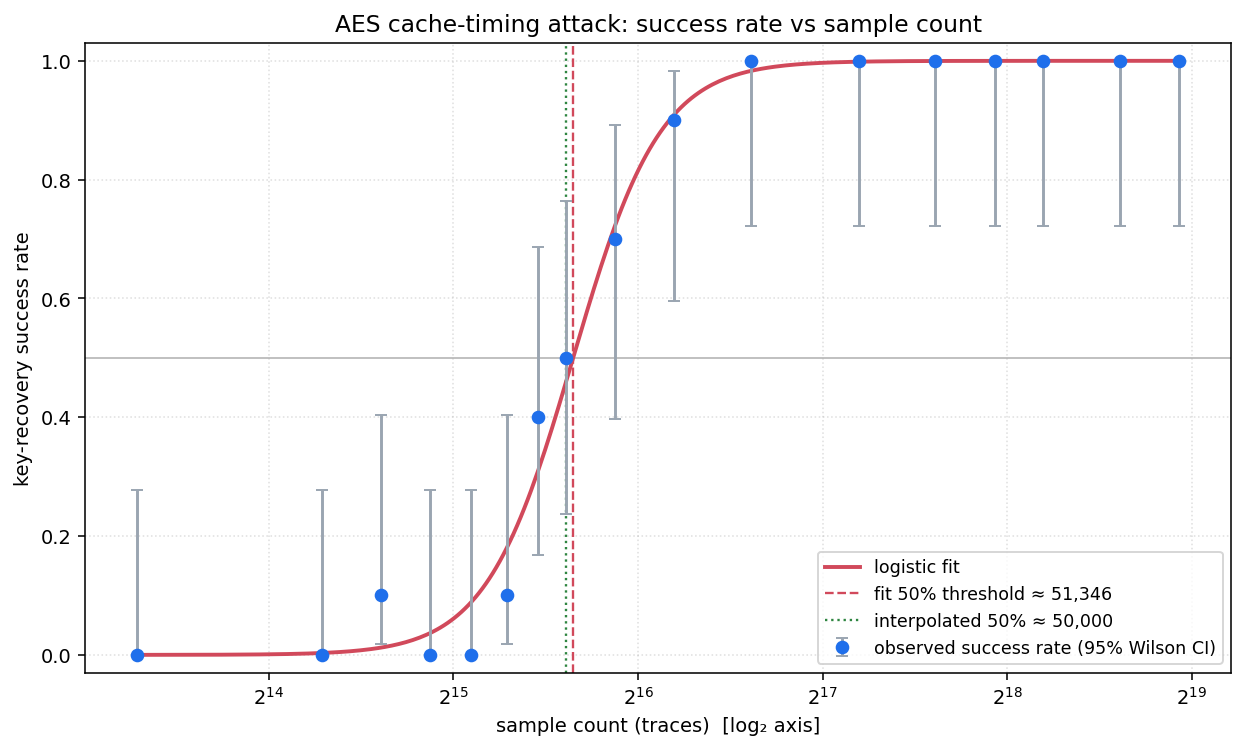
\includegraphics[width=0.82\linewidth]{go_10x_success_rate.png}
\caption{C key-recovery success rate vs.\ trace count (log$_2$ axis) with 95\%
Wilson intervals, the fitted logistic curve, and the 50\% threshold
($N_{50}\approx 51{,}346$).}
\label{fig:c-success}
\end{figure}

Across all counts the mean $t_{\min}$ stays within 112--121 ticks and the mean
score within $\approx17{,}200$--$17{,}460$, with no trend
(Fig.~\ref{fig:covar}). The per-trace leak is unchanged; only the stability of
the group-mean estimates improves with count. The threshold is therefore a
statistical averaging effect, not a signal cliff.

\begin{figure}[t]
\centering
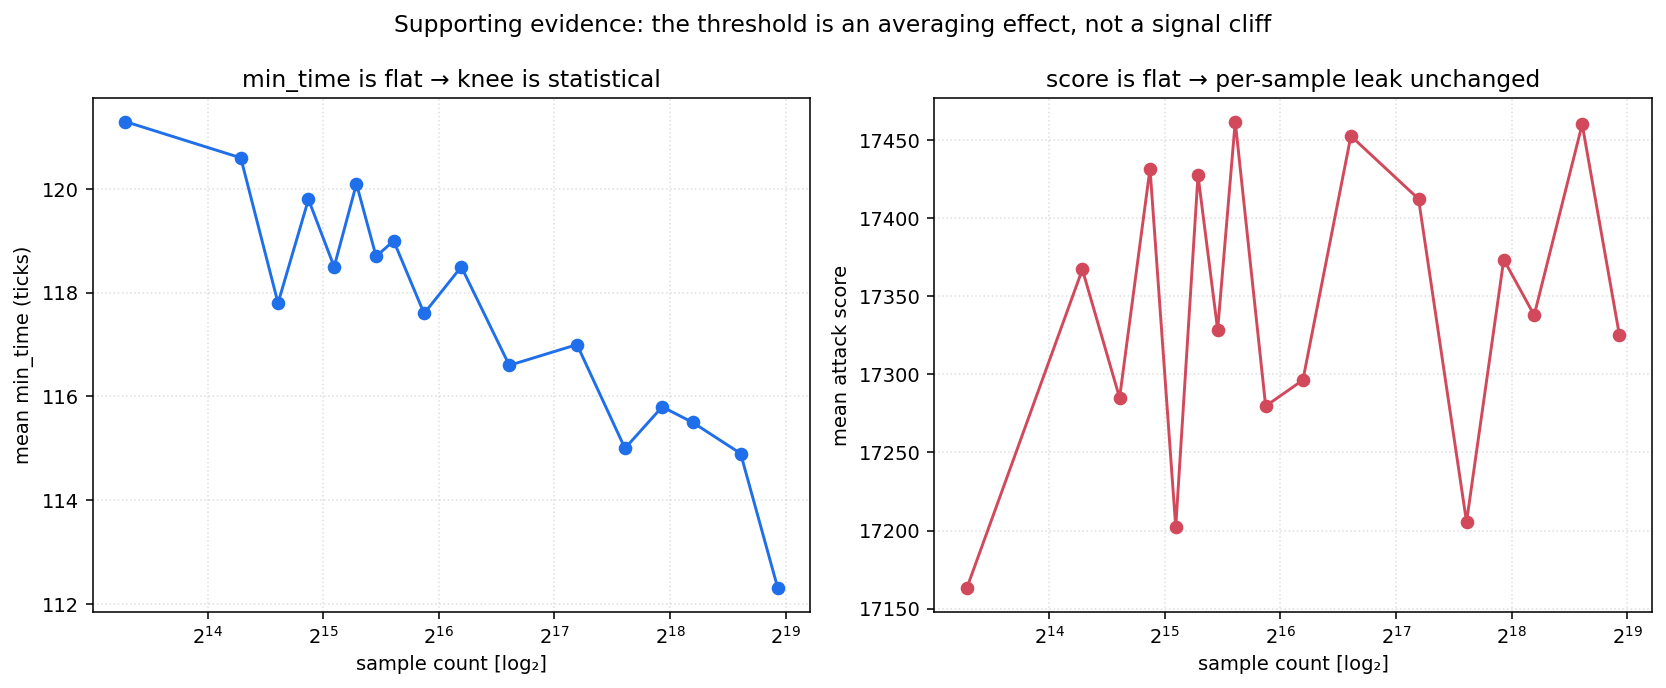
\includegraphics[width=\linewidth]{go_10x_covariates.png}
\caption{Mean $t_{\min}$ (left) and mean attack score (right) are flat across
trace count: the per-trace leak does not change, so the threshold reflects
averaging quality rather than a signal cliff.}
\label{fig:covar}
\end{figure}

\subsection{Cross-language recovery}
\label{sec:res-crosslang}
Under identical counts, key, dials, and recovery logic, the implementations reach
50\% recovery at very different counts (Table~\ref{tab:crosslang},
Fig.~\ref{fig:crosslang}). Go with the garbage collector enabled requires
$N_{50}\approx265{,}283$ ($2^{18.0}$)---about $5.2\times$ the C threshold.

\begin{table}[t]
\centering
\caption{Fitted 50\% trace threshold by implementation (identical parameters).}
\label{tab:crosslang}
\begin{tabular}{lccc}
\toprule
Implementation & $N_{50}$ (traces) & $\log_2 N_{50}$ & Ratio to C \\
\midrule
C           & 51{,}346  & 15.65 & 1.0$\times$ \\
Go (GC on)  & 265{,}283 & 18.02 & 5.2$\times$ \\
Go (GC off) & 243{,}335 & 17.89 & 4.7$\times$ \\
\bottomrule
\end{tabular}
\end{table}

\begin{figure}[t]
\centering
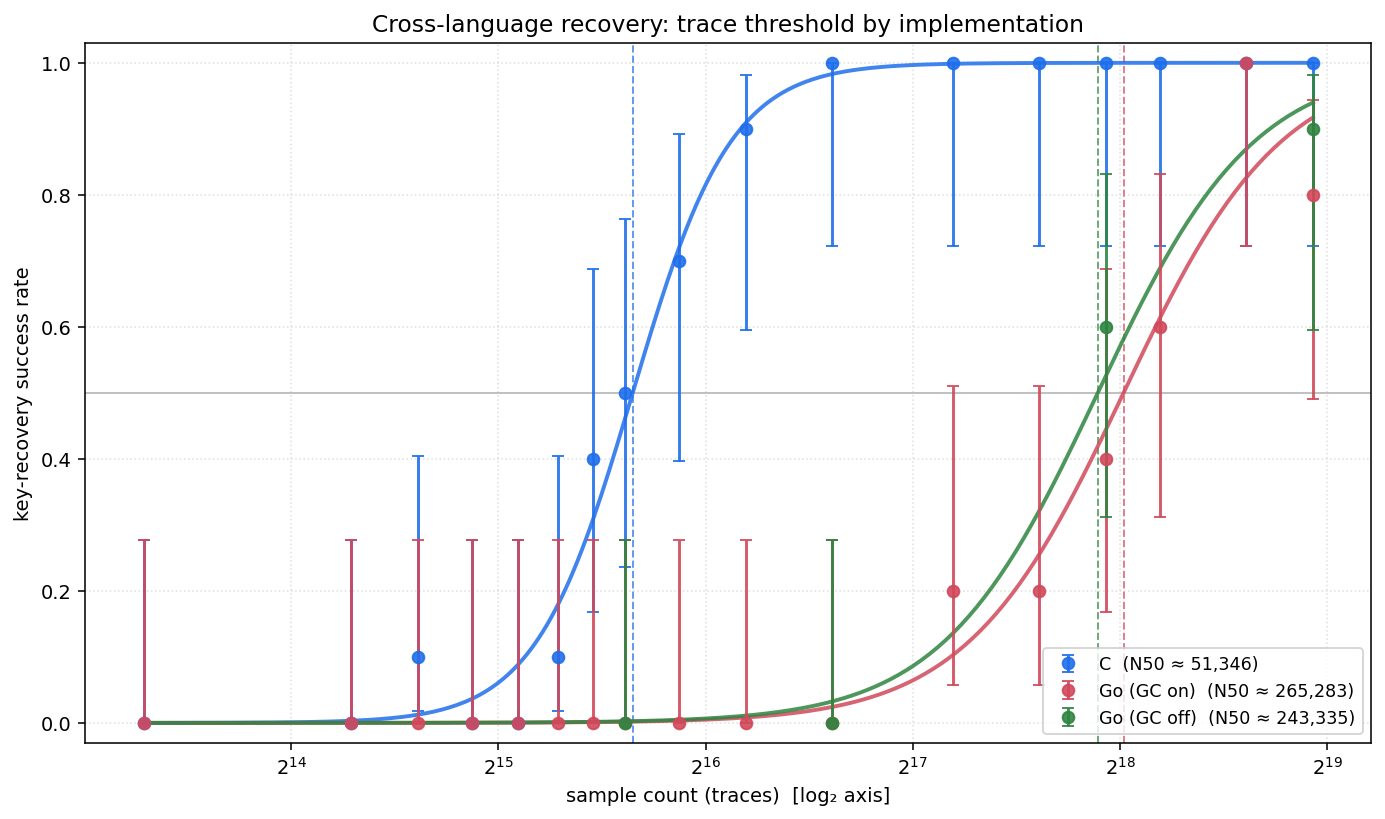
\includegraphics[width=\linewidth]{cross_language_recovery.png}
\caption{Cross-language recovery. C (blue) reaches 50\% recovery near 50k traces;
Go with the collector on (red) and off (green) require roughly five times as
many, their curves nearly coincident. Points show 95\% Wilson intervals; dashed
lines mark each fitted $N_{50}$.}
\label{fig:crosslang}
\end{figure}

\subsection{Runtime-noise ablation (Go, GC on vs.\ off)}
\label{sec:res-gc}
Disabling the collector and pinning one core lowers the fitted threshold only
marginally, from $N_{50}\approx265$k to $\approx243$k ($\approx8\%$), well inside
the sampling uncertainty. At matched counts the GC-off run is equal or slightly
better everywhere (Table~\ref{tab:gc}), but the $\approx5\times$ gap to C is
essentially untouched.

\begin{table}[t]
\centering
\caption{Go recovery at matched counts, garbage collector on vs.\ off
(10 trials each).}
\label{tab:gc}
\begin{tabular}{rcc}
\toprule
Traces & GC on & GC off \\
\midrule
500{,}000 & 8/10 & 9/10 \\
250{,}000 & 4/10 & 6/10 \\
100{,}000 & 0/10 & 0/10 \\
50{,}000  & 0/10 & 0/10 \\
\bottomrule
\end{tabular}
\end{table}

\subsection{Dial sweep}
\label{sec:res-dial}
At 100k traces, increasing \texttt{-repeat} beyond the $r{=}50$ baseline does not
improve C recovery and appears to reduce it, while the strongest disturbance
$e{=}4096$\,KiB gives the highest recovery (Table~\ref{tab:dial},
Fig.~\ref{fig:dial}). With wide $n{=}10$ intervals, the robust reading is that
signal strength (\texttt{-evict-kb}) matters more than additional averaging
(\texttt{-repeat}) at this count. The Go dial sweep is uninformative by
construction: 100k lies far below Go's $\approx265$k threshold, so recovery is
$\approx0$ (1/110 with GC on, 1/60 with GC off) regardless of dial---a
consequence of fixing the dial count at C's knee.

\begin{table}[t]
\centering
\caption{C dial sweep at 100k traces (10 trials each). Left: \texttt{-repeat} at
$e{=}2048$. Right: \texttt{-evict-kb} at $r{=}50$.}
\label{tab:dial}
\begin{tabular}{rc@{\hskip 2em}rc}
\toprule
\texttt{-repeat} & Rate & \texttt{-evict-kb} & Rate \\
\midrule
10  & 60\% & 256  & 80\%  \\
20  & 50\% & 512  & 60\%  \\
30  & 50\% & 1024 & 10\%  \\
50  & 70\% & 2048 & 50\%  \\
75  & 20\% & 4096 & 100\% \\
100 & 20\% &      &       \\
\bottomrule
\end{tabular}
\end{table}

\begin{figure}[t]
\centering
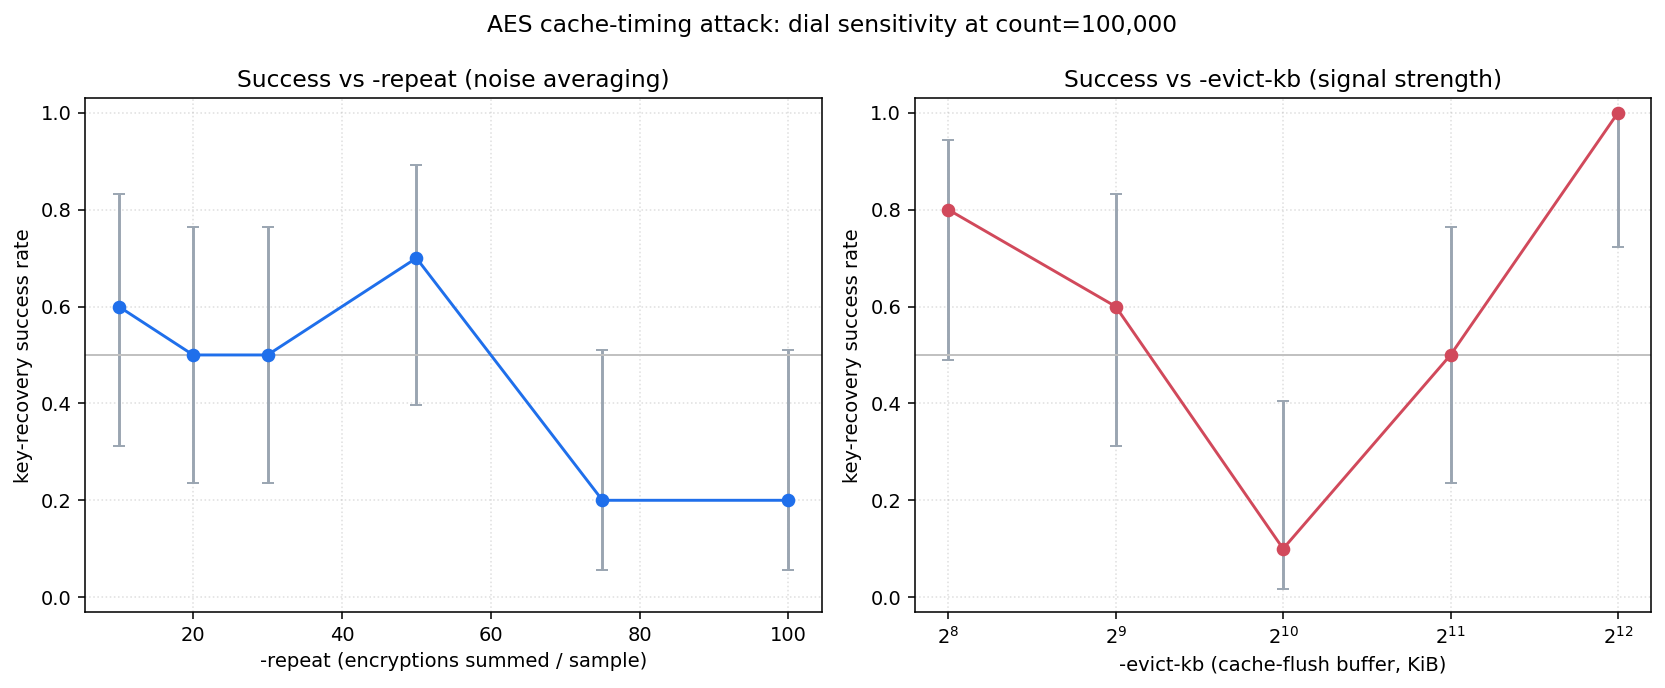
\includegraphics[width=\linewidth]{knee100k_dials.png}
\caption{C dial sweep at 100k traces: recovery vs.\ \texttt{-repeat} (left) and
vs.\ \texttt{-evict-kb} (right), with 95\% Wilson intervals.}
\label{fig:dial}
\end{figure}

\subsection{Cross-language cost and timer normalisation}
\label{sec:res-cost}
Table~\ref{tab:cost} reports per-stage cost measured on the idle machine, with
per-encryption time normalised to nanoseconds using each port's timer
(Sec.~\ref{sec:method-collect}). Mean collection wall-time is comparable for C
and Go (both dominated by the 2\,MiB eviction read), and Go's per-encryption time
is only $\approx2.4\times$ C's once the C tick is converted. Python is far
slower: $\approx55\times$ C in collection and $\approx1800\times$ in the attack,
with a per-encryption time of $\approx42\,\mu$s ($\approx420\times$ C).

\begin{table}[t]
\centering
\caption{Per-stage cost (Apple M4, $r{=}50$, $e{=}2048$). Per-encryption from
$t_{\min}$, with C ticks converted at 41.67\,ns/tick.}
\label{tab:cost}
\begin{tabular}{lcccc}
\toprule
Impl & Timer & Collect (ms/sample) & Attack (ms/sample) & Per-enc.\ (ns) \\
\midrule
C      & \texttt{mach\_absolute\_time} & 0.93 & 0.008 & 99 \\
Go     & \texttt{time.Since().Nanoseconds} & 0.84 & 0.013 & 235 \\
Python & \texttt{perf\_counter\_ns} & 51.3 & 14.6 & 41{,}894 \\
\bottomrule
\end{tabular}
\end{table}

\subsection{Python feasibility}
\label{sec:res-python}
Combining Python's collection and attack costs ($\approx65.9$\,ms per sample),
Table~\ref{tab:python} extrapolates representative workloads. Even a single trial
at C's threshold ($50$k) takes $\approx55$ minutes---and would very likely fail,
since $50$k lies far below Python's own (higher) threshold. Reaching counts near
Go's threshold costs hours per trial, and a full 17-count, 10-trial
characterisation (the design used for C and Go) would take $\approx17$ days of
continuous computation. No Python trial in our probing recovered a key.

\begin{table}[t]
\centering
\caption{Extrapolated pure-Python wall-clock cost ($\approx65.9$\,ms/sample,
collection $+$ attack).}
\label{tab:python}
\begin{tabular}{lc}
\toprule
Workload & Estimated time \\
\midrule
One trial at 50{,}000 traces (C's $N_{50}$)   & $\approx 55$ min \\
One trial at 265{,}000 traces (Go's $N_{50}$) & $\approx 4.9$ h \\
Full 17-count $\times$ 10-trial sweep         & $\approx 17$ days \\
\bottomrule
\end{tabular}
\end{table}

% ===========================================================================
\section{Analysis and Discussion}
\label{sec:analysis}

\subsection{The threshold is an averaging effect}
\label{sec:an-statistical}
The flatness of $t_{\min}$ and score across count localises the mechanism. The
per-trace cache-collision signal is a fixed quantity independent of how many
traces are collected; what changes with count is the variance of each group mean
$T_{i,j}[d]$. With more traces per ciphertext-difference group, the correct
final-round relation separates from the noise floor more reliably, so recovery is
a smooth, probabilistic function of count---hence the psychometric curve rather
than a hard boundary. This also explains why the threshold is best summarised by
a fitted $N_{50}$ with confidence intervals rather than a single ``required''
count.

\subsection{Why Go needs about five times more traces}
\label{sec:an-crosslang}
The same attack, on the same key, recovers with $\approx5\times$ more traces in
Go than in C. Because the recovery logic is common, the difference originates in
collection. The timer-normalised costs (Table~\ref{tab:cost}) show that Go's
\emph{mean} per-encryption time is only $\approx2.4\times$ C's---far short of the
$5\times$ threshold gap---so the gap is not explained by mean overhead but by the
\emph{variance} of Go's measurements: a noisier estimate of the same signal
requires more traces to average down. The garbage-collector ablation
(Sec.~\ref{sec:res-gc}) sharpens this: if GC pauses were the dominant noise,
disabling the collector would move the threshold substantially; instead it moves
$N_{50}$ by $\approx8\%$ and leaves the gap intact. The residual noise is
therefore the broader managed-runtime measurement path---bounds-checked array
access, scheduler quanta, and higher-overhead timing---rather than the collector
specifically. In short, Go's disadvantage is real, reproducible, and a property
of \emph{measurement}, and it persists after the most obvious runtime lever is
removed.

\subsection{Dials: signal strength over averaging, and a design lesson}
\label{sec:an-dial}
Within C at the 100k knee, additional \texttt{-repeat} does not help and the
largest \texttt{-evict-kb} helps most, consistent with the averaging/signal
split: near threshold the binding constraint is per-trace signal strength
(improved by stronger eviction), not additional averaging, and very large
\texttt{-repeat} may lengthen each measurement enough to admit more
environmental perturbation. The Go dial sweep carries a methodological lesson
rather than a result: fixing the dial count at C's knee ($100$k) placed it below
Go's operating threshold ($\approx265$k), so the sweep could not probe Go's dial
sensitivity. A fair cross-language dial comparison would choose each
implementation's dial count relative to its own threshold.

\subsection{Python is infeasible, not merely slow}
\label{sec:an-python}
Python's cost (Table~\ref{tab:cost},~\ref{tab:python}) makes measured recovery
impractical on this platform: a full characterisation would take on the order of
weeks. Worse, the same interpreter overhead that inflates the mean
($\approx420\times$ per encryption) also inflates measurement variance, so
Python's trace threshold is expected to exceed even Go's---placing verified
recovery beyond any feasible trace budget rather than merely expensive. Python
therefore remains valuable as a readable reference for algorithmic consistency
but is unsuitable as a measured-timing collector, a conclusion that follows from
runtime cost alone.

\subsection{Positioning against prior work}
\label{sec:an-prior}
Bonneau and Mironov's expanded final-round attack recovers from a median of
$2^{13}$--$2^{14.3}$ samples under cache eviction on 2006
hardware~\cite{bonneau06}. Our C threshold ($N_{50}\approx2^{15.6}$; high
reliability $\approx2^{16.2}$) is roughly one order of magnitude higher. This is
expected rather than contradictory: the comparison mixes algorithm with platform
and instrument---their hardware cycle counters on a Pentium III/UltraSPARC versus
our aggregate wall-clock timing on an Apple M4 with a different cache hierarchy
and coarser timer. Agreement to within an order of magnitude on entirely
different hardware indicates the leakage mechanism reproduces as predicted; the
absolute count is a property of the platform and instrument.

\subsection{Threats to validity}
\label{sec:an-threats}
\begin{itemize}
  \item \textbf{Single key.} All runs reuse one fixed key to isolate trace count;
        thresholds may vary across keys.
  \item \textbf{Sampling uncertainty.} Ten trials per count give wide Wilson
        intervals near 0/10 and 10/10; individual dial points should not be
        over-interpreted, and $N_{50}$ is an estimate.
  \item \textbf{Environment sensitivity.} Independent clean C sweeps place the
        threshold near 50k and 100k and a contaminated sweep near 150k; the
        threshold is sensitive to background load, which we control by an
        environment gate but cannot eliminate on a general-purpose machine.
  \item \textbf{Native-collection confound.} The cross-language comparison uses
        each language's own traces (different seeds), so it isolates
        runtime-in-collection, not shared-dataset algorithmic consistency.
  \item \textbf{Reduced ablation grid and platform confound.} The GC-off grid is
        coarse, and the prior-work comparison spans different hardware eras; both
        are stated where used.
\end{itemize}

% ===========================================================================
\section{Conclusion and Future Work}
\label{sec:conclusion}

We measured the trace-count threshold of a final-round cache-collision attack on
a modern Apple M4 and, holding the algorithm fixed, quantified how the
implementation runtime performing the collection changes that threshold. The C
implementation recovers with a fitted 50\% threshold near $51$k traces; the same
attack collected in Go's managed runtime needs about five times as many, and a
garbage-collector ablation shows that this gap is broad measurement noise rather
than GC pauses---after timer-unit normalisation, Go's mean per-encryption cost is
only $\approx2.4\times$ C's, so the gap is variance-driven. Pure-Python measured
recovery is infeasible on this platform by cost alone. The overarching finding is
that the practical cost of a cache-timing attack depends materially on the
implementation runtime, not only on the algorithm.

Two directions remain open. First, a \emph{shared-dataset} consistency and
performance study: supply one trace file to all three ports to confirm identical
verified-key recovery and to compare stage-level processing time without
differing collection noise. Second, broaden generalisation with multiple keys,
alternative outlier rules (percentile trimming, median absolute deviation), and a
per-implementation dial calibration so dial sensitivity can be compared across
languages at each port's own operating point.

% ===========================================================================
\appendix
\section{Dataset provenance and exclusions}
\label{app:prov}
All runs share commit \texttt{405b3de} (harness modified in place) and one fixed
key. Table~\ref{tab:prov} lists the included runs; excluded runs are the
contaminated earliest C sweep ($\approx3.0$\,ms/sample) and exploratory
pilots (fewer trials, missing sidecars, or single-point grids), retained with
metadata for audit. The canonical C run is stored under a
\texttt{go}-prefixed filename for historical reasons but is verified C
(Sec.~\ref{sec:method-governance}).

\begin{table}[t]
\centering
\caption{Included runs (Apple M4; 10 trials/point; interleaved; $r{=}50$,
$e{=}2048$ unless noted).}
\label{tab:prov}
\begin{tabular}{llcc}
\toprule
Role & Impl & Seed & Recovery \\
\midrule
C count (canonical)  & C  & 4175  & 97/170 \\
C count (replicate)  & C  & 10053 & 64/170 \\
C dial (100k)        & C  & 11065 & 57/110 \\
Go count (GC on)     & Go & 14778 & 32/170 \\
Go dial (GC on)      & Go & 20346 & 1/110  \\
Go count (GC off)    & Go & 9744  & 15/40  \\
Go dial (GC off)     & Go & 31480 & 1/60   \\
\bottomrule
\end{tabular}
\end{table}

\bibliographystyle{ieeetr}
\bibliography{references}

\end{document}
